% !TeX spellcheck = en_US
\addscenariosection{1}{Cooperative Scenario}{Emerald Island}{\images/logistics.png}

\begin{multicols*}{2}

\textbf{Author:} Invoceusse

\textbf{Source:} \href{https://discord.com/channels/740870068178649108/1222679455261261986}{Archon Studio Discord}

\textit{Lord Markham has decided to organize a treasure hunt and you and your friends are going to take part.
  But hurry up! Other teams are also on the trail, and one of them is almost finished!
  And above all, beware: it seems that a creature identified as a dragon lurks on this island!}
\subsection*{\MakeUppercase{Scenario Length}}

This Scenario is played over 8 Rounds.

\subsection*{\MakeUppercase{Player Setup}}

\textbf{Player Count:} 1 -- 4

\textbf{Starting Resources:} 5 \svg{gold}, 2 \svg{building_materials}, 1 \svg{valuables}

\textbf{Starting Income:} 10 \svg{gold}, 0 \svg{building_materials}, 1 \svg{valuables}

\textbf{Starting Units:}
\begin{itemize}
  \item A Pack of \svgunit{bronze} Units of your choice
  \item A Few \svgunit{bronze} Units of your choice
\end{itemize}

\textbf{Town Buildings:} \svgunit{bronze} Dwelling

\textbf{Map Tile Pool:} If you wish, you can distribute the II--III Tiles equally to each player rather than laying them out as proposed.

\textbf{Additional Bonus:} None

\subsection*{\MakeUppercase{Map Setup}}

Take the following Map Tiles and arrange them as shown in the Scenario map layout ($P$ stands for the number of players):

\begin{itemize}
  \item P × Starting (I) Map Tile
  \item 4P × Far (II--III) Map Tile
\end{itemize}

\subsection*{\MakeUppercase{Victory Conditions}}

Flag all Mines and Settlements. (Don't forget the Building Materials Mine in Tile I. Each Tile II--III contains one Mine or Settlement with a Level III fight.)

\subsection*{\MakeUppercase{Defeat Conditions}}

There are unflagged Mines or Settlements left in map at the end of Round 8.

\subsection*{\MakeUppercase{Timed Events}}

\textbf{\nth{5} Round:}
\begin{itemize}
  \item Gain again the result of one Field with a Black Cube.
\end{itemize}

\subsection*{\MakeUppercase{Additional Rules}}

\begin{itemize}
    \item Ignore any yellow lines between Tiles I (but not between Tiles I and Tiles II--III).

    \item You can't build a \svgunit{golden} Dwelling.

    \item You can give Units to another player, even outside your Turn, if one of your Heroes is:
    \begin{itemize}
        \item On the same Map Tile as another player's Hero.
        \item In another player's Town.
        \item Next to another player's Hero.
    \end{itemize}

    \item If you have no Units in your Unit Deck (after a battle or if you do not keep at least one Unit), return all your Units to your Faction's Unit pool (even if another player has one or more of your Units). This includes Units you've previously given to another player.

    \item When in another player's Town, you may Recruit or Reinforce their Units, either for them or for yourself. You need the other player's permission for it. Corresponding Dwellings or Citadel must be built to do so.

    \item For the last Mine/Settlement battle, add a \svgunit{golden} Neutral Unit. You have unlimited Turns for this battle. You can't use Expert Diplomacy to skip this battle!

    \item The first time you reach Level IV, gain your second specialty.

    \item When you reach Level IV, move your Token on the Level tracker to Level III.

    \item Additionally, no player can:
    \begin{itemize}
        \item Attack other Heroes.
        \item Capture a Mine or Settlement that is already Flagged.
    \end{itemize}
\end{itemize}

\vspace{2em}

\begin{center}
  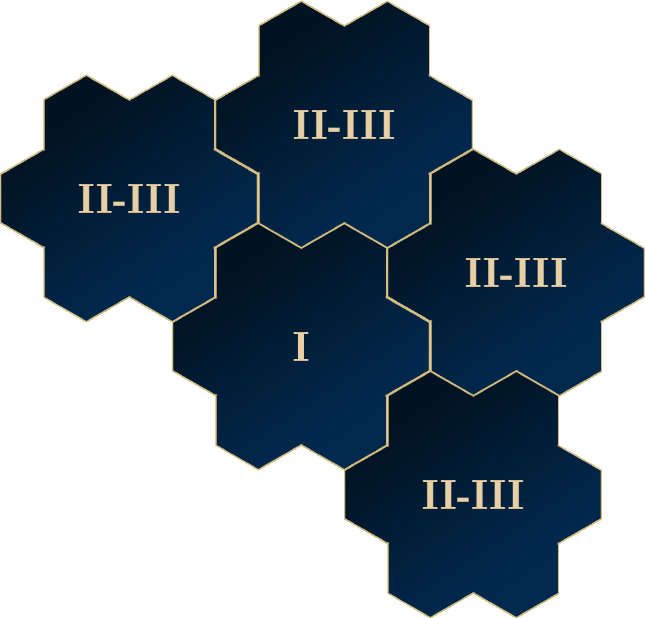
\includegraphics[width=0.2\paperwidth]{\maps/emerald-1.png}
  \captionof{figure}{\textbf{1-PLAYER SCENARIO}}
  \vspace{3em}
  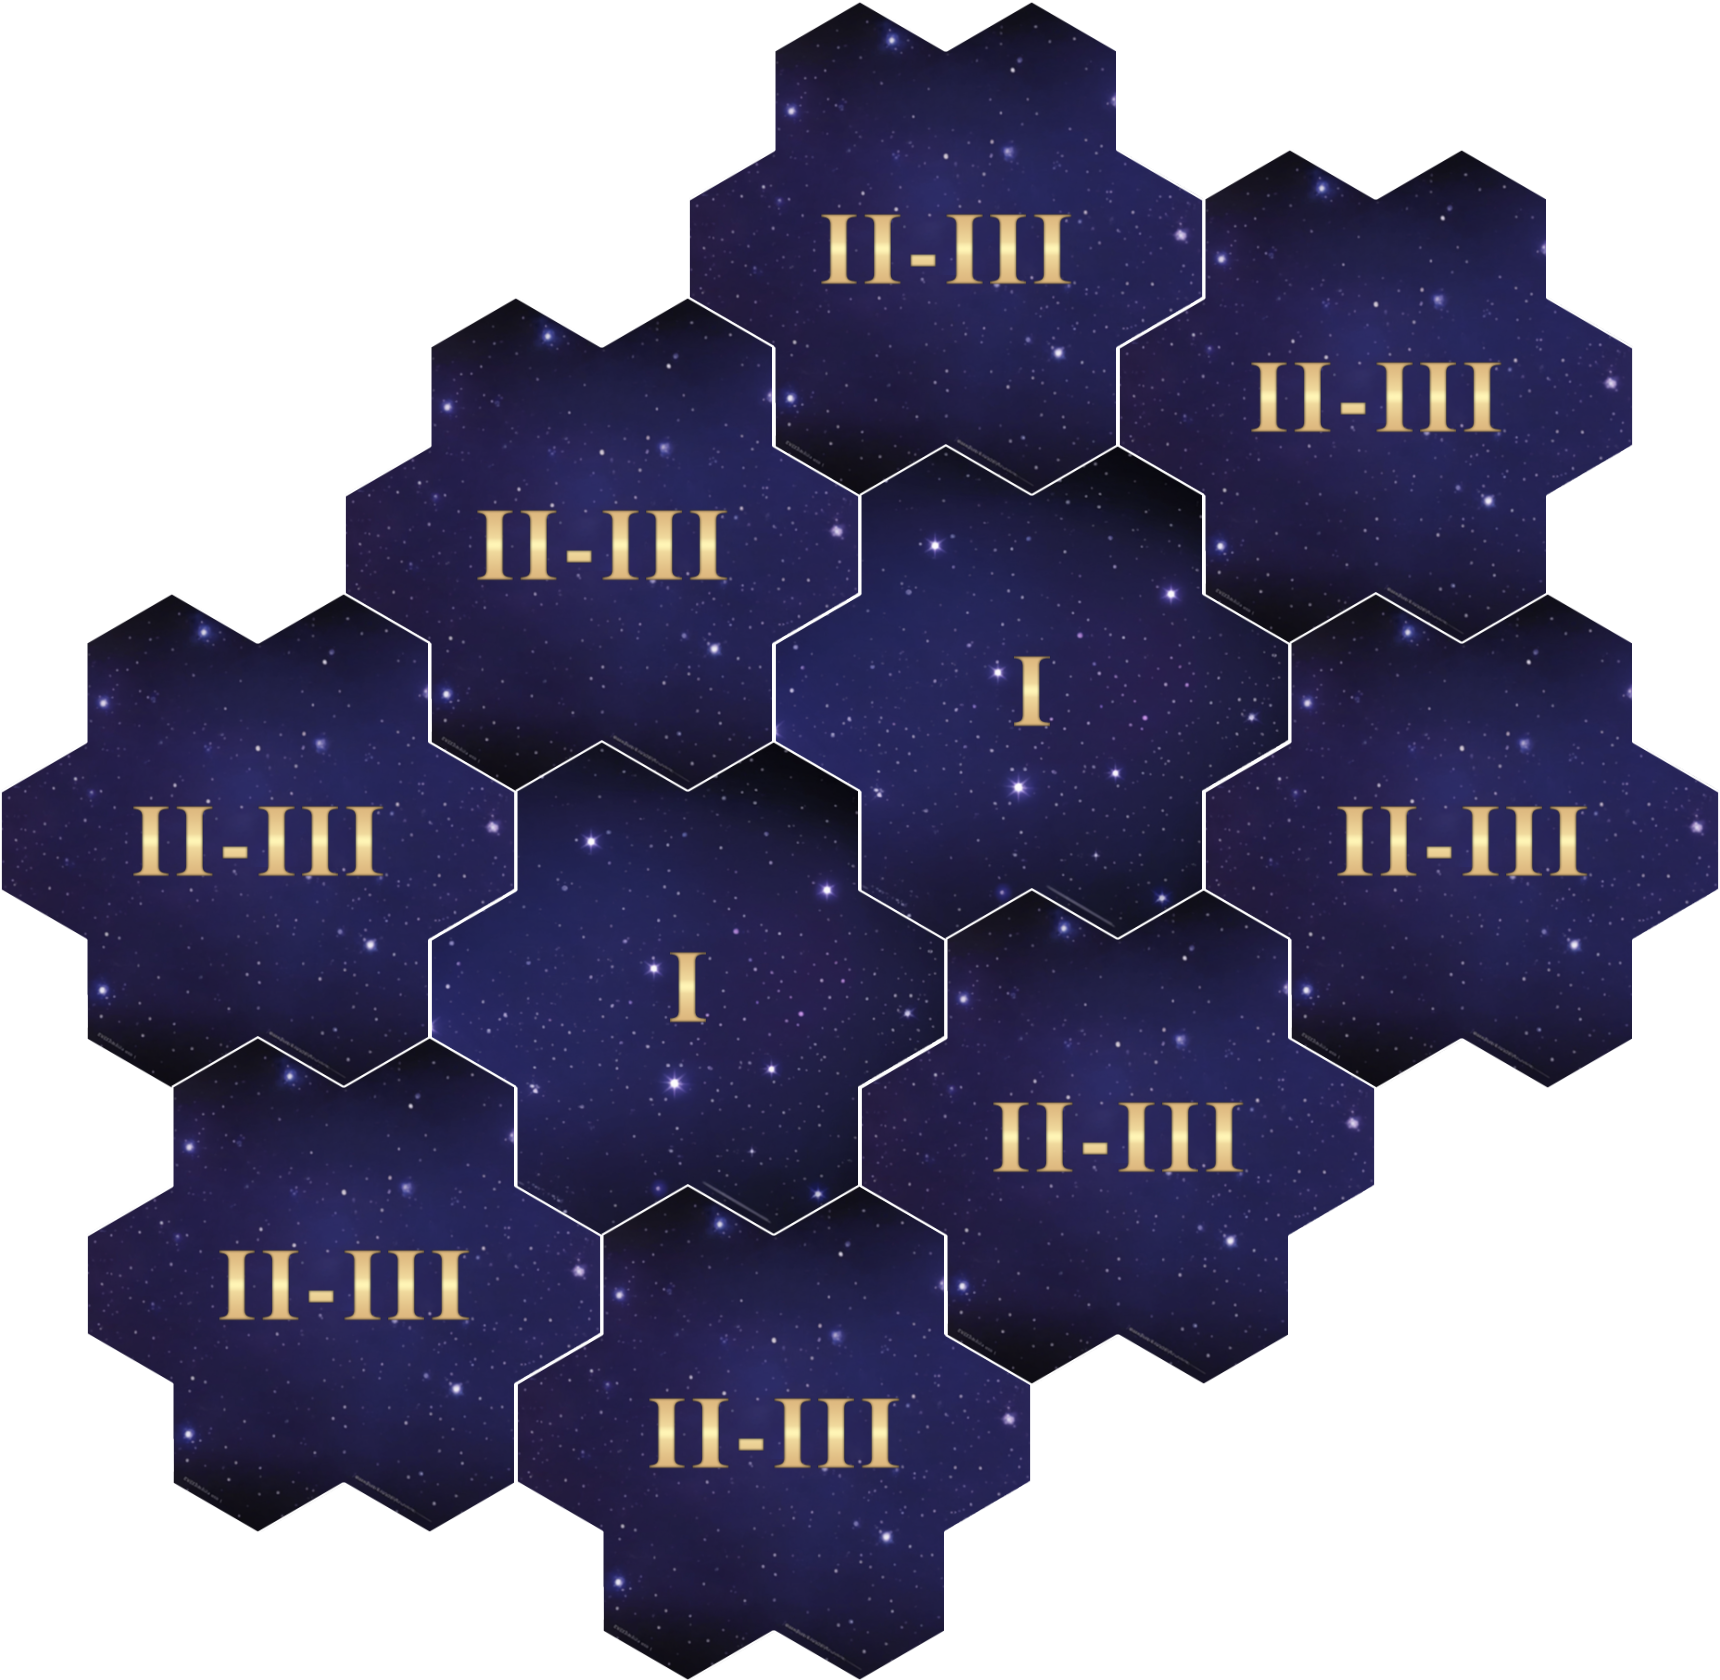
\includegraphics[width=0.3\paperwidth]{\maps/emerald-2.png}
  \captionof{figure}{\textbf{2-PLAYER SCENARIO}}
  \vspace{3em}
  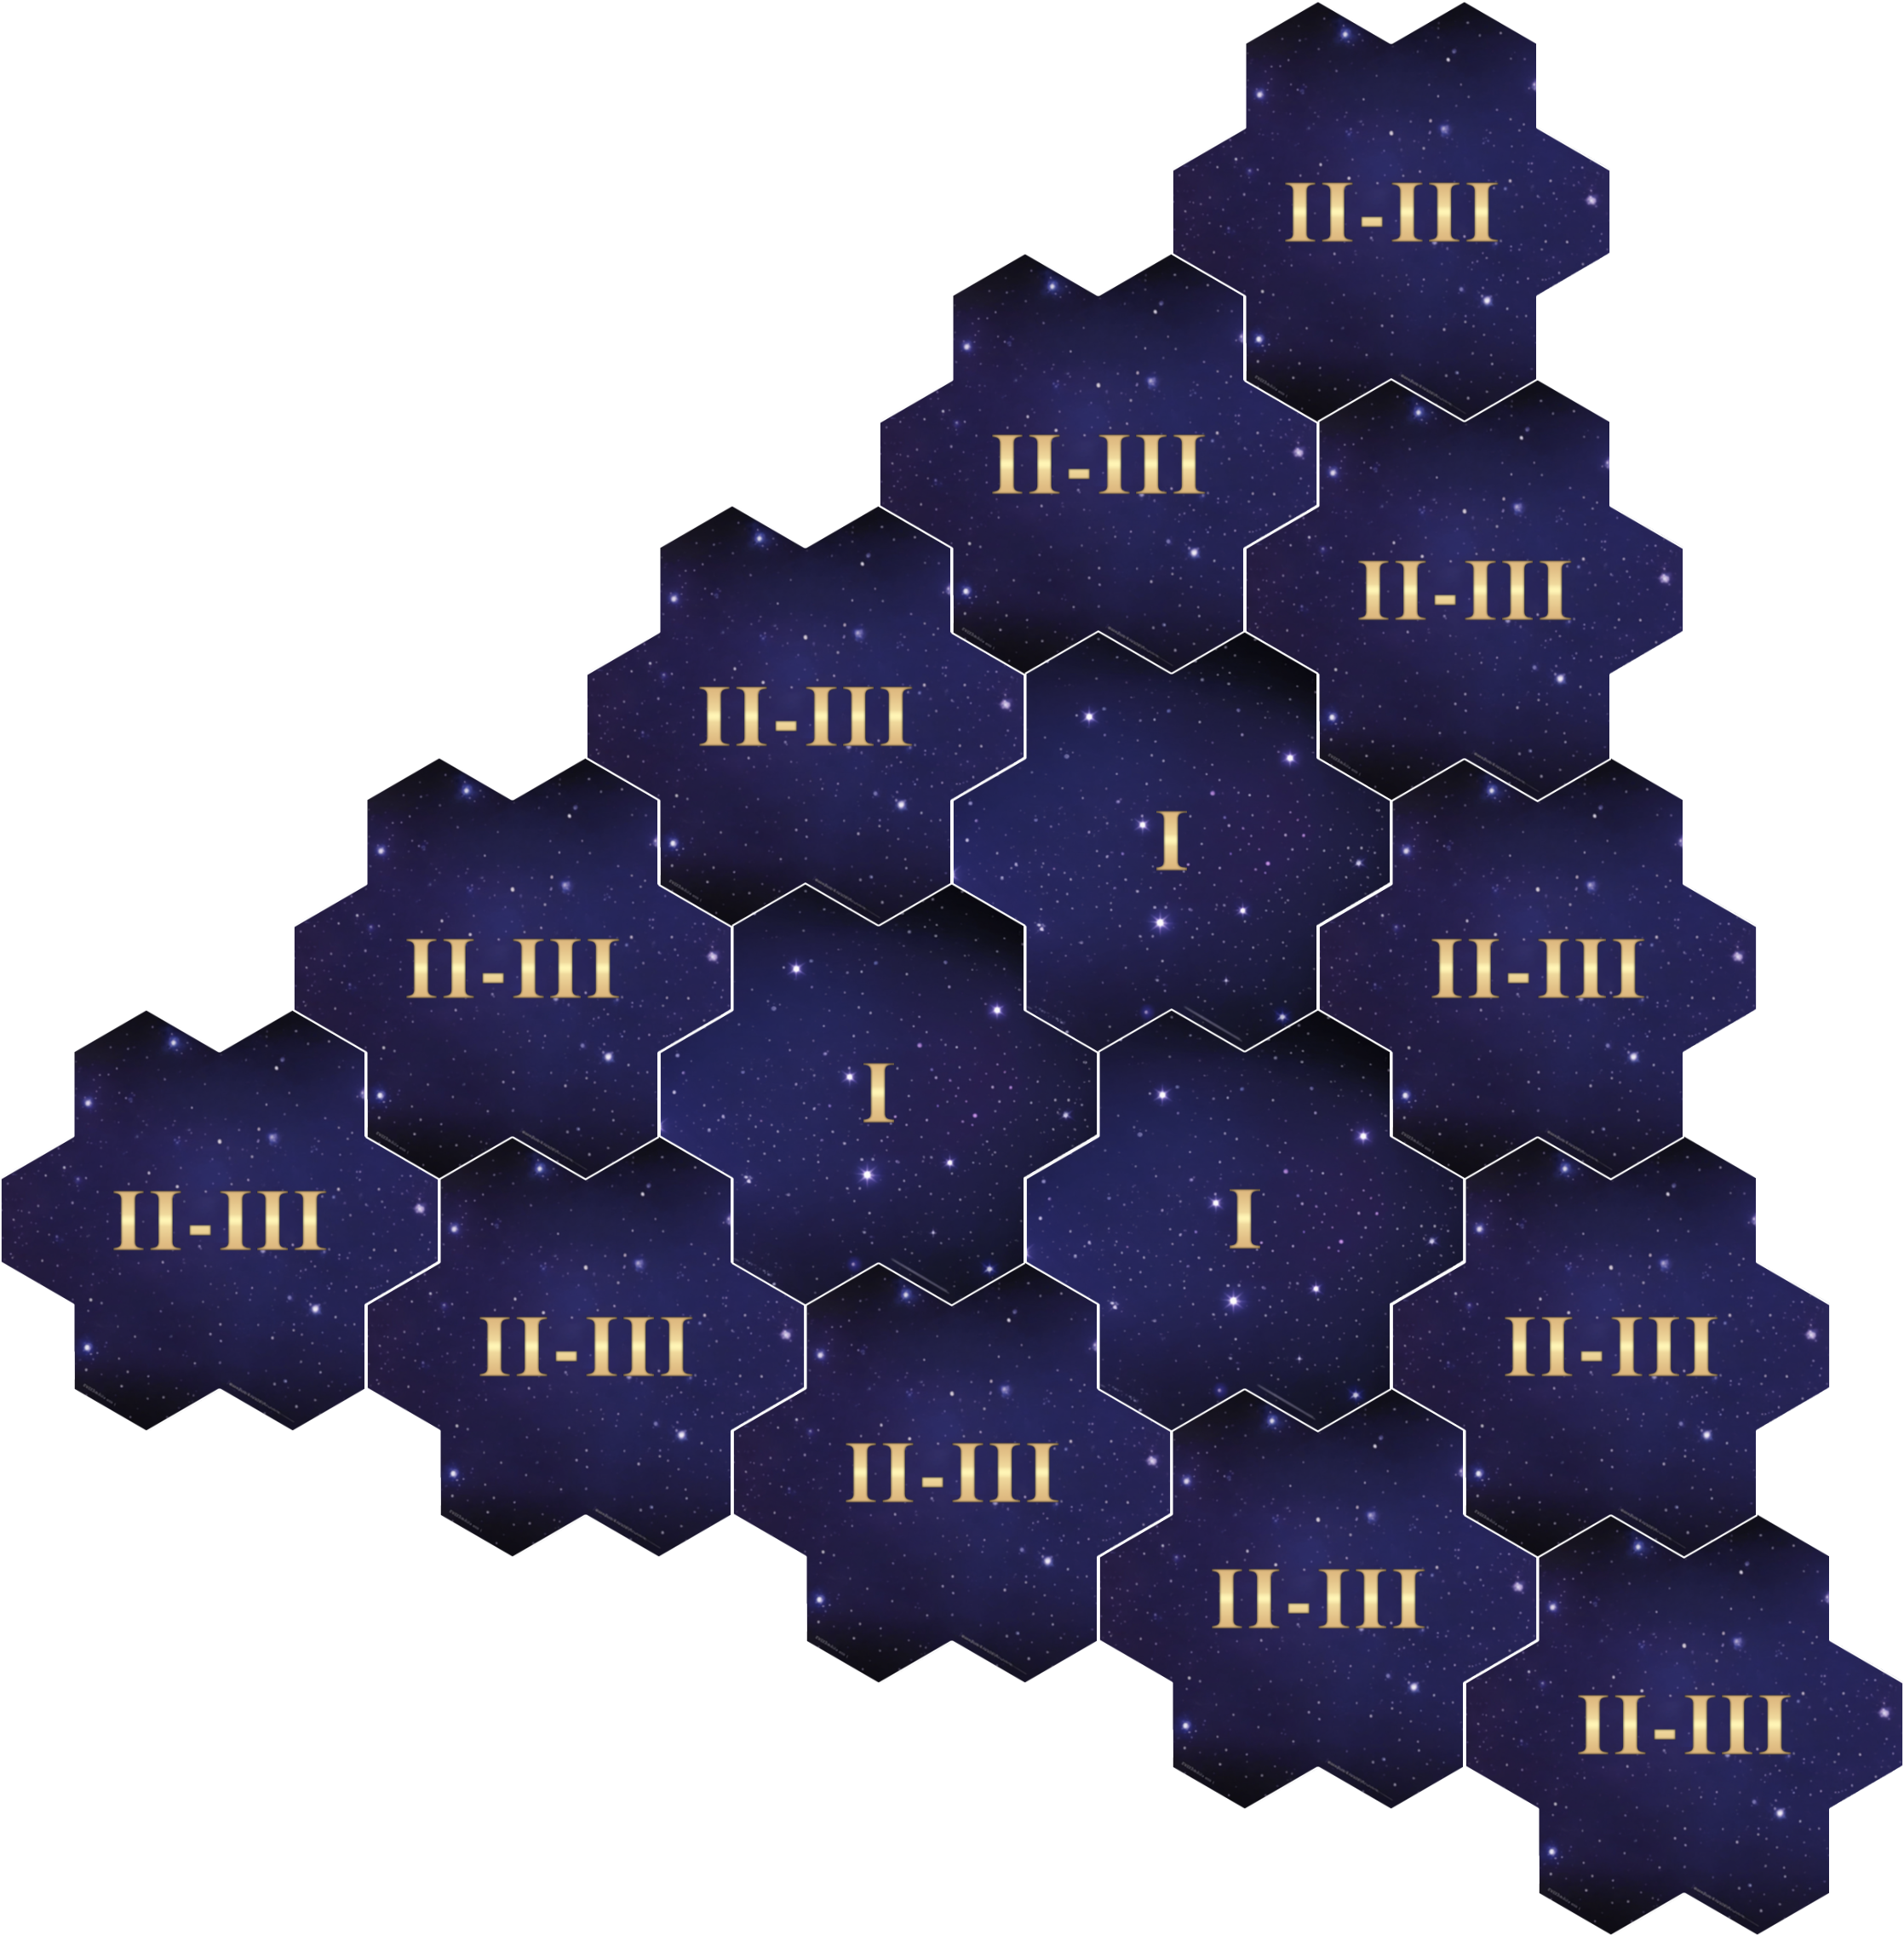
\includegraphics[width=0.3\paperwidth]{\maps/emerald-3.png}
  \captionof{figure}{\textbf{3-PLAYER SCENARIO}}
  \vspace{3em}
  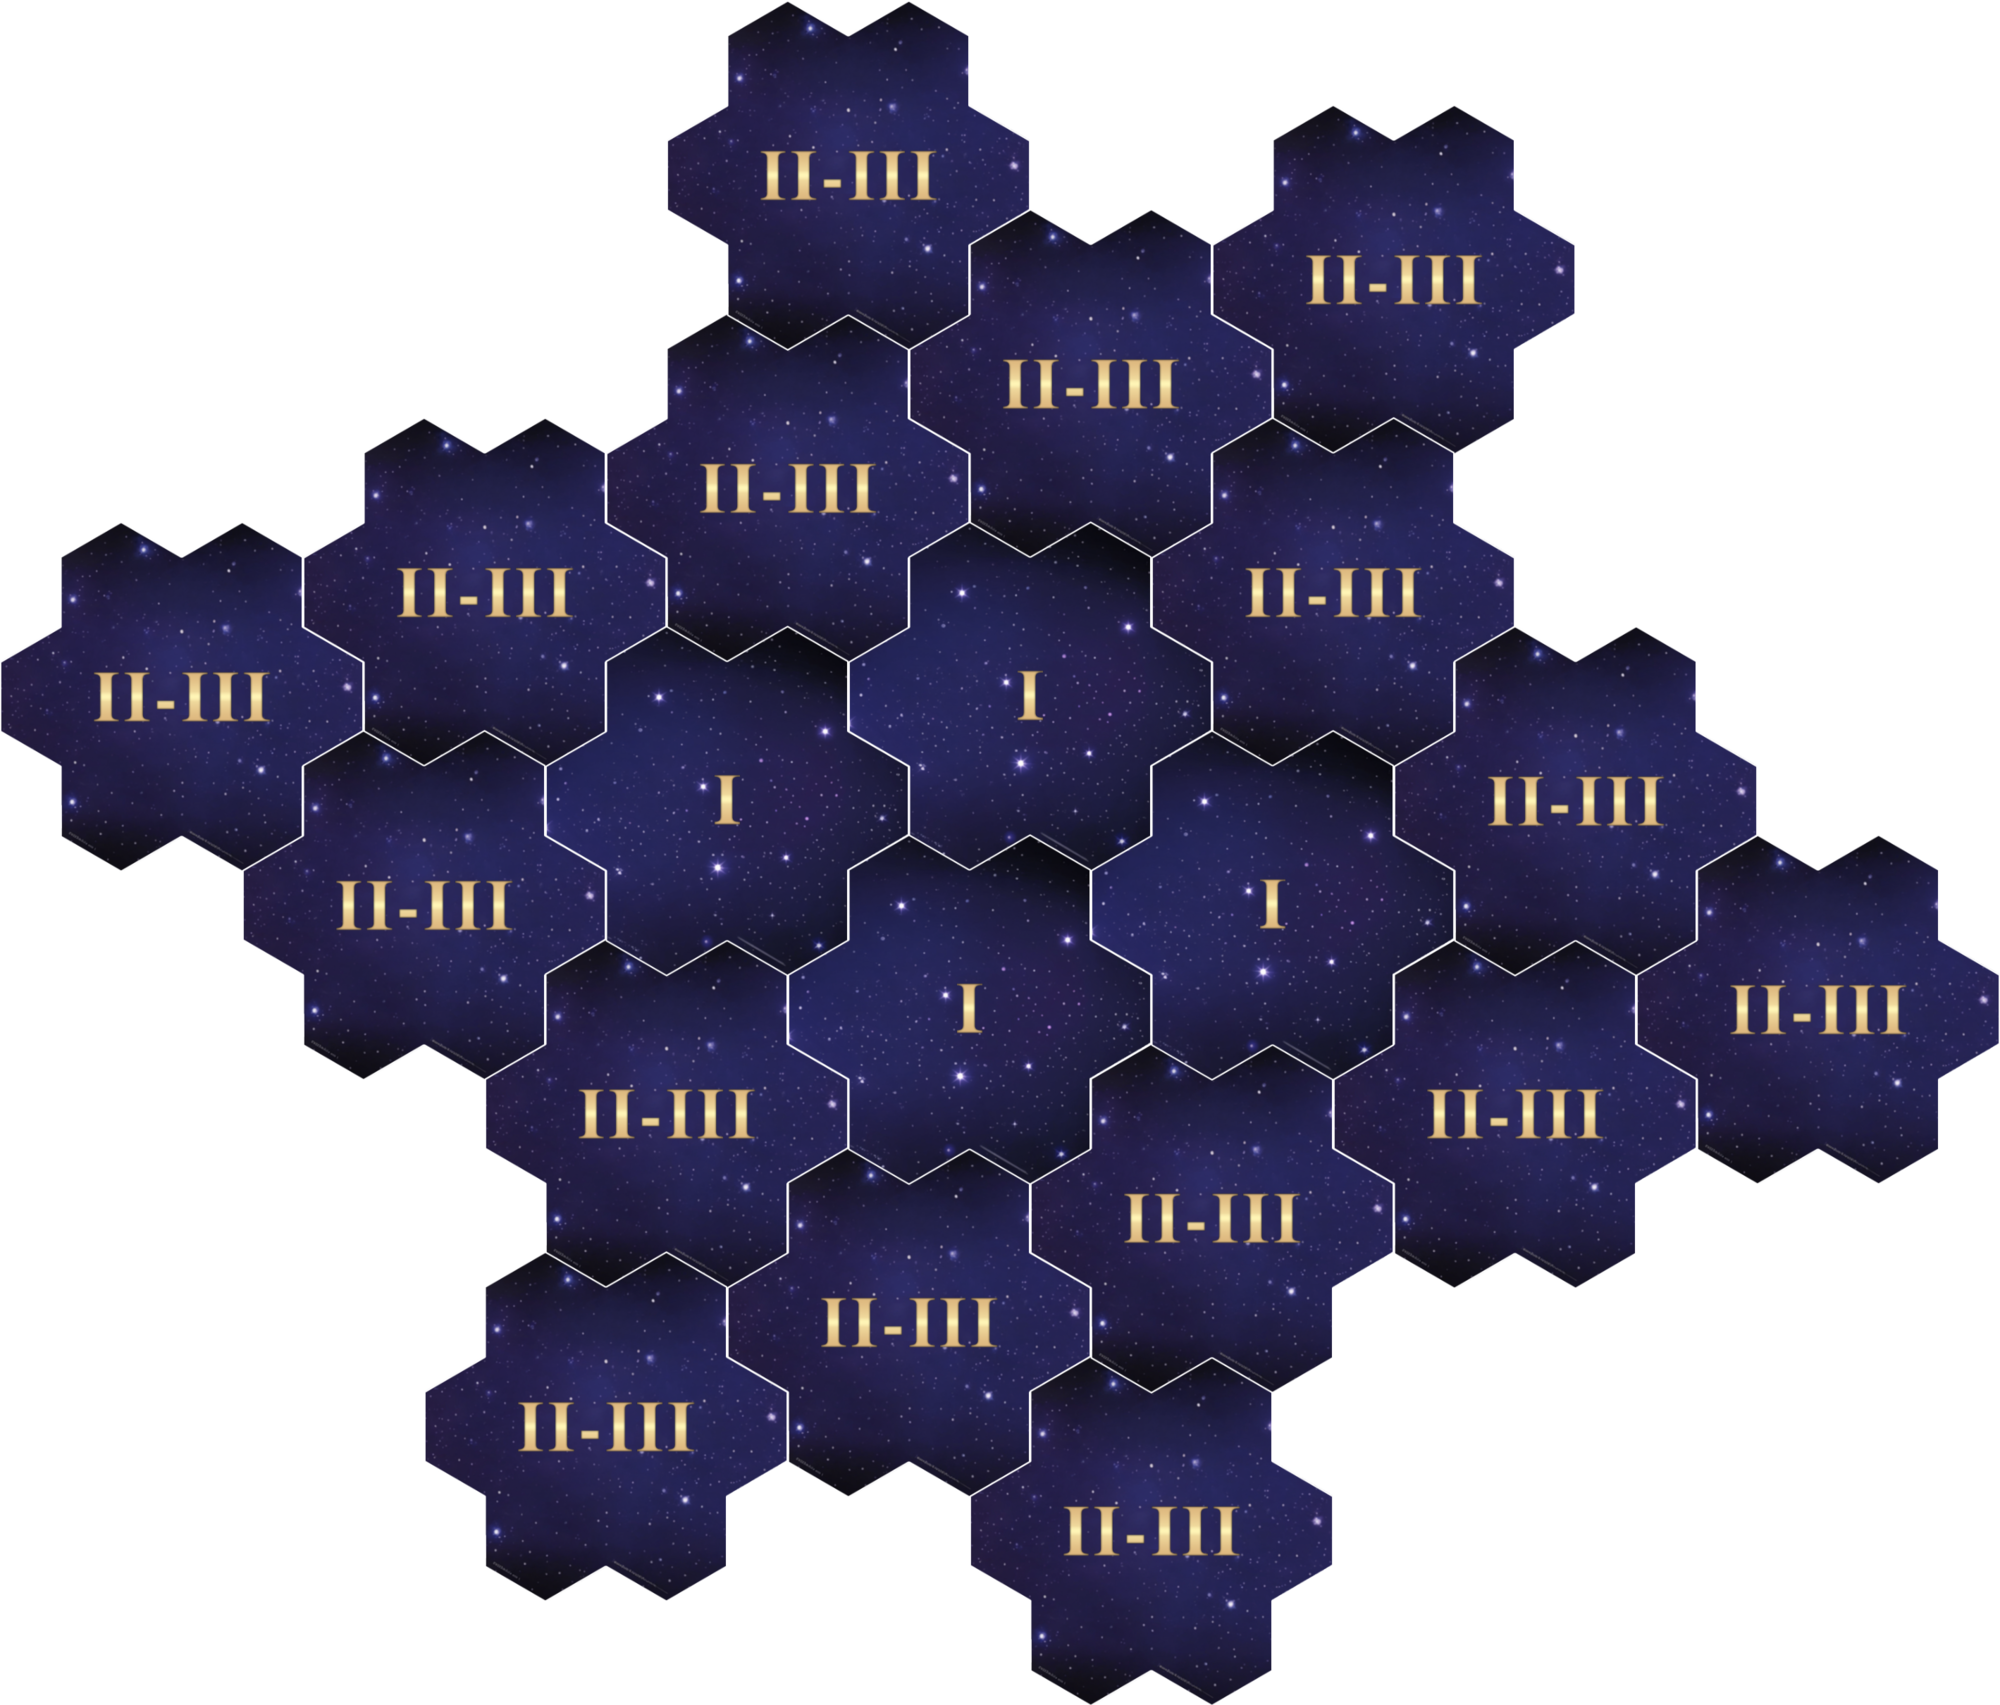
\includegraphics[width=0.3\paperwidth]{\maps/emerald-4.png}
  \captionof{figure}{\textbf{4-PLAYER SCENARIO}}
\end{center}

\end{multicols*}
